\section{第三章 离散信源}

\begin{remarkBox}{本章重点}
本章主要回答“信源内部的统计结构是什么”这件事。学习时先抓住离散信源的分类与模型，再理解无记忆信源扩展、平稳信源熵率、马尔可夫链与马尔可夫信源，最后把“相关性”“剩余度”和“效率”联系起来。
\end{remarkBox}

\subsection{离散信源的分类与数学模型}

\subsubsection{离散信源的分类}
离散信源是输出符号取离散值的信源。按不同角度可以分为：

\begin{definitionBox}{离散信源分类}
离散信源常按以下方式分类：
\begin{itemize}
  \item 按符号取值：\textbf{离散信源}与\textbf{连续信源}；
  \item 按记忆性：\textbf{无记忆信源}与\textbf{有记忆信源}；
  \item 按符号集规模：\textbf{有限离散信源}与\textbf{无限离散信源}；
  \item 按统计特性：\textbf{平稳信源}与\textbf{非平稳信源}。
\end{itemize}
\end{definitionBox}

\begin{center}
\begin{tikzpicture}[
    scale=0.92,
    level 1/.style={sibling distance=3.8cm, level distance=1.6cm},
    level 2/.style={sibling distance=2.2cm, level distance=1.3cm},
    box/.style={draw, thick, rounded corners=2pt, minimum width=1.8cm, minimum height=0.6cm, align=center, font=\small},
    leaf/.style={box, minimum width=1.2cm}
  ]
  \node[box, fill=MidnightBlue!10, draw=MidnightBlue!60!black, font=\bfseries] {离散信源\\分类}
    child { node[box, fill=RoyalBlue!10, draw=RoyalBlue!50!black] {按符号取值}
      child { node[leaf, fill=RoyalBlue!6] {离散} }
      child { node[leaf, fill=RoyalBlue!6] {连续} }
    }
    child { node[box, fill=SeaGreen!10, draw=SeaGreen!50!black] {按记忆性}
      child { node[leaf, fill=SeaGreen!6] {无记忆} }
      child { node[leaf, fill=SeaGreen!6] {有记忆} }
    }
    child { node[box, fill=Orange!10, draw=Orange!50!black] {按统计特性}
      child { node[leaf, fill=Orange!6] {平稳} }
      child { node[leaf, fill=Orange!6] {非平稳} }
    };
\end{tikzpicture}
\end{center}

\begin{keypoint}{分类的意义}
分类不是为了记名字，而是为了判断后面该用哪种熵、哪种扩展模型、哪种状态转移描述。
\end{keypoint}

\subsubsection{单符号离散无记忆信源模型}
离散无记忆信源每次输出的符号相互独立，且每个符号的概率分布固定。

\begin{definitionBox}{单符号离散无记忆信源}
设符号集 $A=\{a_1,\dots,a_n\}$，若
\[
 p(a_i)\ge 0,\qquad \sum_{i=1}^n p(a_i)=1,
\]
则称其为一个离散无记忆信源的单符号模型。
\end{definitionBox}

\begin{formulaBox}{无记忆信源的联合概率}
若 $X_1,\dots,X_N$ 相互独立，则
\[
 p(x_1,\dots,x_N)=\prod_{k=1}^N p(x_k).
\]
\end{formulaBox}

无记忆信源是最简单的信源模型——各次输出独立，联合概率直接拆成乘积。这意味着我们不需要考虑符号之间的依赖关系，熵的计算也最简单。但现实中几乎不存在完全无记忆的信源，它更多是一个理想化的起点：其他更复杂的模型（平稳信源、马氏信源）可以看作在无记忆基础上逐步引入依赖关系。

\subsubsection{多维离散无记忆信源}
当我们需要同时考虑信源连续输出的多个符号时，不能只靠单符号模型。扩展源把一组连续输出看成一个整体，这样就能用我们已有的熵工具来研究序列。

\begin{definitionBox}{$N$ 次扩展源}
把信源连续输出的 $N$ 个符号组成向量 $X^N=(X_1,\dots,X_N)$，称为信源的 $N$ 次扩展。
\end{definitionBox}

\begin{warningBox}{扩展源的直觉}
扩展不是“把公式乘上 $N$”这么简单，而是把一次输出变成一个长度为 $N$ 的序列，再研究这个序列整体的熵。
\end{warningBox}

例如，一个二元无记忆信源的三次扩展源，符号集变成了 $\{000,001,010,011,100,101,110,111\}$ 共 $2^3=8$ 个符号——符号数随 $N$ 指数增长，但每个新符号的概率由独立性直接相乘得到，熵则按定理 3.1 线性增长。这两点（联合概率可拆、熵线性增长）是无记忆信源最重要的计算特征。

\subsubsection{平稳信源}
平稳信源的统计特性与时间平移无关。

\begin{definitionBox}{离散平稳信源}
若对任意 $i_1,\dots,i_N,h,j_1,\dots,j_N$，都有
\[
 p(x_{i_1}=a_{j_1},\dots,x_{i_N}=a_{j_N})
 =
 p(x_{i_1+h}=a_{j_1},\dots,x_{i_N+h}=a_{j_N}),
\]
则称该信源为离散平稳信源。
\end{definitionBox}

\begin{formulaBox}{平稳信源的等价形式}
平稳性也可写成
\[
 p(x_{i_1},x_{i_2},\dots,x_{i_N})
 =
 p(x_{i_1+h},x_{i_2+h},\dots,x_{i_N+h}).
\]
对连续片段，有
\[
 p(x_i,x_{i+1},\dots,x_{i+N})
 =
 p(x_j,x_{j+1},\dots,x_{j+N}).
\]
因此对应的条件概率与熵也不随时间起点改变：
\[
 P(x_{i+N}\mid x_i,x_{i+1},\dots,x_{i+N-1})
 =
 P(x_{j+N}\mid x_j,x_{j+1},\dots,x_{j+N-1}),
\]
\[
 H(X_iX_{i+1}\cdots X_{i+N})
 =
 H(X_jX_{j+1}\cdots X_{j+N}).
\]
\end{formulaBox}

\begin{keypoint}{平稳性的意义}
平稳信源的“未来”和“过去”在统计意义上没有区别，所以可以讨论长期平均的符号熵，也就是熵率。
\end{keypoint}

\subsubsection{平稳信源的平均符号熵与熵率}
对平稳信源，我们往往不关心某一次特定输出的熵，而是想回答一个更实际的问题：长期看来，这个信源每输出一个符号，平均携带多少信息？这就引出了平均符号熵和熵率。

\begin{definitionBox}{平均符号熵}
对长度为 $N$ 的信源序列，定义平均符号熵为
\[
 H_N(X)=\frac{1}{N}H(X^N).
\]
\end{definitionBox}

\begin{definitionBox}{熵率}
若极限存在，则定义
\[
 H_\infty(X)=\lim_{N\to\infty}\frac{1}{N}H(X^N)
\]
为信源的熵率。
\end{definitionBox}

平均符号熵和熵率本质上在回答同一个问题——序列越长，每个符号平均多少信息——但角度不同：$H_N(X)$ 是有限 $N$ 的近似，$H_\infty(X)$ 是 $N\to\infty$ 的极限。考试中，无记忆信源直接有 $H_\infty=H(X)$；有记忆信源则需要通过条件熵或平稳分布来求。

\begin{formulaBox}{熵率的理解}
$H_\infty(X)$ 表示信源长序列下每个符号平均携带的信息量。无记忆时它等于单符号熵；有相关性时它一般更小。
\end{formulaBox}

\begin{formulaBox}{有记忆信源的扩展熵上界}
对平稳有记忆信源，通常有
\[
 H(X^N)\le N H(X_1),
\]
等号当且仅当各符号相互独立，即退化为无记忆信源。
\end{formulaBox}

\subsection{离散无记忆信源的扩展}

无记忆信源最核心的性质是定理 3.1：扩展熵等于单符号熵乘以扩展次数。这个定理虽然简单，但它是整个扩展源理论的基石，也是判断"信源是否有记忆"的一个试金石——如果扩展熵不成比例，就说明存在依赖关系。

\begin{theoremBox}{定理3.1：无记忆信源的扩展熵}
若 $X$ 是离散无记忆信源，则它的 $N$ 次扩展源熵满足
\[
 H(X^N)=N H(X).
\]
\end{theoremBox}

\begin{proof}
由于无记忆信源的各次输出相互独立，联合熵可由链式法则化为各单符号熵之和，因此 $H(X^N)=\sum_{k=1}^N H(X_k)=N H(X)$。
\end{proof}

\begin{keypoint}{这一定理在做什么}
它告诉我们：只要信源无记忆，扩展多少次，平均每个符号携带的信息量都不变。
\end{keypoint}

\begin{example}
\label{ex:binary-memoryless}
\textbf{二元无记忆信源}：设 $A=\{0,1\}$，$P(X=0)=p$，$P(X=1)=q=1-p$。求单符号熵和二次扩展源熵。

\noindent \textbf{解题流程}：\\[2pt]
步骤一：先写出单符号分布。\\
步骤二：代入熵公式 $H(X)=-p\log p-q\log q$。\\
步骤三：利用定理3.1 得到 $H(X^2)=2H(X)$。

\textbf{解}：
\[
H(X)=-p\log p-q\log q=-p\log p-(1-p)\log(1-p).
\]
因此
\[
H(X^2)=2H(X).
\]
\end{example}

\begin{example}
\textbf{二次扩展模型}：求上例中信源的二次扩展模型。

\noindent \textbf{解题流程}：\\[2pt]
步骤一：写出二次扩展符号集 $\{00,01,10,11\}$。\\
步骤二：由于无记忆，各对符号的概率等于对应单符号概率乘积。\\
步骤三：核对概率和是否为 1。

\textbf{解}：
\[
P(00)=p^2,\quad P(01)=pq,\quad P(10)=qp,\quad P(11)=q^2.
\]
\end{example}

\begin{example}
\textbf{二元信源熵}：设 $q=1-p$，则
\[
H(X)=-p\log p-q\log q=-p\log p-(1-p)\log(1-p)=H(p).
\]
\end{example}

\begin{example}
\label{ex:extension-entropy}
\textbf{二次扩展源熵}：给定 $P=[1/2,1/4,1/4]$，求二次扩展源熵。

\noindent \textbf{解题流程}：\\[2pt]
步骤一：先求单符号熵 $H(X)$。\\
步骤二：用无记忆扩展公式 $H(X^2)=2H(X)$。\\
步骤三：写出单位说明。

\textbf{解}：
\[
H(X)=-\frac12\log\frac12-\frac14\log\frac14-\frac14\log\frac14=\frac32\text{ bit}.
\]
所以
\[
H(X^2)=2H(X)=3\text{ bit/2个符号}.
\]
\end{example}

\subsection{离散平稳信源的熵}

有了平稳信源的定义和熵率的概念，现在来看平稳信源的几个核心数学结论。定理 3.3 是本章最深刻的结果之一——它用条件熵给出了熵率的一个等价定义，同时也证明了平均符号熵的单调递减性。

\begin{theoremBox}{定理3.3：平稳信源熵的单调性与极限}
任意离散平稳信源，若 $H_1(X)<\infty$，则
\[
 H(X_N\mid X_1\cdots X_{N-1})
\]
随 $N$ 非增；并且
\[
 H_N(X)\ge H(X_N\mid X_1\cdots X_{N-1}),
\]
\[
 H_N(X)\le H_{N-1}(X),
\]
\[
 H_\infty(X)=\lim_{N\to\infty}H(X_N\mid X_1\cdots X_{N-1}).
\]
\end{theoremBox}

\begin{keypoint}{平稳信源的核心结论}
平稳信源的平均符号熵会随着扩展长度增加而下降，并最终收敛到熵率。相关性越强，熵率越低。
\end{keypoint}

\begin{formulaBox}{平稳信源的熵阶梯}
\[
 H_0\ge H_1\ge H_2\ge\cdots\ge H_\infty.
\]
这里 $H_0=\log |A|$ 是同一符号集上的等概最大熵参考值；$H_N(X)=H(X^N)/N$ 是 $N\ge1$ 时的平均符号熵，$H_\infty$ 对应长序列极限平均信息量。
\end{formulaBox}

\begin{example}
\textbf{平稳信源的边缘分布}：设平稳信源 $A=\{0,1\}$，已知 $P(x_1=0)=p$，求 $P(x_n=0),P(x_n=1)$ 及相关条件概率的关系。

\noindent \textbf{解题流程}：\\[2pt]
步骤一：利用平稳性，任意时刻的边缘分布相同。\\
步骤二：写出 $P(x_n=0)=P(x_1=0)=p$。\\
步骤三：补充说明条件概率由平稳统计结构决定，而不是由时间位置决定。

\textbf{解}：
\[
P(x_n=0)=p,\qquad P(x_n=1)=1-p.
\]
因为信源平稳，所以不同时间位置的边缘分布相同。
\end{example}

\subsection{有限状态马尔可夫链}

\subsubsection{马尔可夫链基本概念}
马尔可夫链是最典型的有记忆随机过程。它的核心思想是：未来只依赖当前状态，而与更早的历史无关。

\begin{definitionBox}{马尔可夫性质}
若随机过程满足
\[
 P(X_{n+1}=x_{n+1}\mid X_n=x_n,\dots,X_1=x_1)=P(X_{n+1}=x_{n+1}\mid X_n=x_n),
\]
则称其满足一阶马尔可夫性质。

\noindent 等号左边是以整个历史为条件的概率，右边仅以当前一步为条件。马尔可夫性质的意思是：已知 $X_n$ 之后，更早的 $X_{n-1},X_{n-2},\dots$ 对预测 $X_{n+1}$ 没有任何额外的帮助——未来与过去在给定现在的条件下独立。
\end{definitionBox}

本章只讨论状态数有限的情况——因为无限状态马氏链的概率和极限行为更复杂，不在课程范围内。

\begin{definitionBox}{有限状态马尔可夫链}
若马尔可夫链的状态集合是有限个状态，则称为有限状态马尔可夫链。
\end{definitionBox}

\begin{formulaBox}{转移概率}
\[
 p_{ij}(m,n)=P(x_n=j\mid x_m=i).
\]
它满足
\[
 0\le p_{ij}(m,n)\le 1,\qquad \sum_j p_{ij}(m,n)=1.
\]
一步转移概率：
\[
 p_{ij}(m,m+1)=P(x_{m+1}=j\mid x_m=i).
\]
\end{formulaBox}

\begin{definitionBox}{齐次马尔可夫链}
若一步转移概率与时刻 $m$ 无关，即
\[
 p_{ij}(m,m+1)=p_{ij},
\]
则称该马尔可夫链为齐次马尔可夫链。其转移矩阵为
\[
 P=(p_{ij}),\qquad p_{ij}\ge0,\quad \sum_j p_{ij}=1.
\]
\end{definitionBox}

下面用一个二元马尔可夫链的例子来直观展示转移概率的含义——状态的自我保持和相互转移都标在箭头上。

\begin{center}
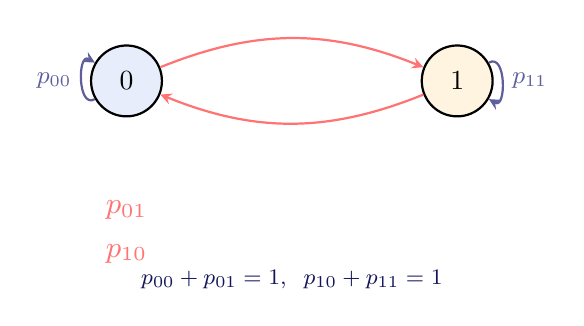
\begin{tikzpicture}[>=stealth, scale=1.2]
  % States
  \node[circle, draw, thick, fill=RoyalBlue!12, minimum size=0.9cm, font=\bfseries] (s0) at (0, 1.6) {$0$};
  \node[circle, draw, thick, fill=Orange!12,   minimum size=0.9cm, font=\bfseries] (s1) at (3.5, 1.6) {$1$};
  % Self-loops
  \draw[->, thick, MidnightBlue!70]
    (s0) .. controls +(-150:0.6) and +(-210:0.6) .. (s0)
    node[midway, left, font=\small] {$p_{00}$};
  \draw[->, thick, MidnightBlue!70]
    (s1) .. controls +(30:0.6) and +(330:0.6) .. (s1)
    node[midway, right, font=\small] {$p_{11}$};
  % Cross transitions with bends
  \draw[->, thick, red!55]
    (s0) to [bend left=22] (s1)
    node[midway, above, font=\small] {$p_{01}$};
  \draw[->, thick, red!55]
    (s1) to [bend left=22] (s0)
    node[midway, below, font=\small] {$p_{10}$};
  % Legend
  \node[font=\footnotesize, MidnightBlue!80!black] at (1.75, -0.5)
    {$p_{00}+p_{01}=1,\;\; p_{10}+p_{11}=1$};
\end{tikzpicture}
\end{center}

\begin{formulaBox}{$k$步与0步转移}
\[
 p_{ij}^{(k)}(m)=P(x_{m+k}=j\mid x_m=i),
\]
\[
 p_{ij}^{(0)}=
\begin{cases}
1,& i=j,\\
0,& i\ne j.
\end{cases}
\]
对齐次马尔可夫链，$k$ 步转移矩阵满足
\[
 P^{(k)}=P^k,\qquad p_{ij}^{(k)}=(P^k)_{ij}.
\]
\end{formulaBox}

\begin{formulaBox}{Kolmogorov-Chapman 方程}
\[
 p_{ij}^{(m+n)}=\sum_k p_{ik}^{(m)}p_{kj}^{(n)}.
\]
矩阵形式为
\[
 P^{(m+n)}=P^{(m)}P^{(n)}.
\]
\end{formulaBox}

K-C 方程的直观含义是：「从 $i$ 出发走 $m+n$ 步到达 $j$，等价于先走 $m$ 步到某个中间状态 $k$，再从 $k$ 走 $n$ 步到 $j$」。这和矩阵乘法的定义完全一致——所以实际计算中直接用矩阵乘法即可，不必逐项展开求和。

\begin{formulaBox}{状态分布递推}
设初始状态分布为
\[
 p^{(0)}=(p_1^{(0)},p_2^{(0)},\dots,p_J^{(0)}),
\]
则齐次马尔可夫链在 $k$ 步后的状态分布为
\[
 p^{(k)}=p^{(0)}P^k,
\]
并且对任意 $m<k$，有
\[
 p^{(k)}=p^{(m)}P^{k-m}.
\]
\end{formulaBox}

\begin{definitionBox}{平稳分布}
若
\[
 P(x_m=i)=P(x_n=i)=\pi_i,
\]
且满足
\[
 \pi_j=\sum_i \pi_i p_{ij},\qquad \pi^T=\pi^T P,
\]
则称 $\pi$ 为该马尔可夫链的平稳分布。
\end{definitionBox}

\begin{keypoint}{平稳分布的作用}
平稳分布告诉你：链长期运行后，各状态出现的稳定比例是多少。
\end{keypoint}

\begin{example}
\textbf{判断转移矩阵}：验证下式是否为齐次马氏链转移矩阵，并确定状态数。
\[
P = \begin{pmatrix}
0.7 & 0.3 \\
0.4 & 0.6
\end{pmatrix}
\]

\noindent \textbf{解题流程}：\\[2pt]
步骤一：检查矩阵是否每行和为 1。\\
步骤二：检查元素是否非负。\\
步骤三：矩阵维数就是状态数。

\noindent \textbf{解}：\\[2pt]
每行和：$0.7+0.3=1$，$0.4+0.6=1$，满足行和为 1。\\
所有元素 $0.7,0.3,0.4,0.6$ 均非负。\\
矩阵为 $2\times2$，故状态数为 2。
\end{example}

\begin{example}
\textbf{一步、两步转移}：求上例中马氏链1步、2步转移后的状态分布，设初始分布 $\pi_0=(0.5,0.5)$。

\noindent \textbf{解题流程}：\\[2pt]
步骤一：先写初始分布向量。\\
步骤二：一步分布由初始分布左乘转移矩阵得到。\\
步骤三：两步分布由转移矩阵平方得到。

\noindent \textbf{解}：\\[2pt]
一步转移后：$\pi_1=\pi_0 P =(0.5,0.5)\begin{pmatrix}0.7&0.3\\0.4&0.6\end{pmatrix}=(0.55,0.45)$。\\[4pt]
两步转移矩阵：$P^2=P\cdot P=\begin{pmatrix}0.7&0.3\\0.4&0.6\end{pmatrix}^2=\begin{pmatrix}0.61&0.39\\0.52&0.48\end{pmatrix}$。\\
两步转移后：$\pi_2=\pi_0 P^2=(0.5,0.5)\begin{pmatrix}0.61&0.39\\0.52&0.48\end{pmatrix}=(0.565,0.435)$。\\[2pt]
或等价地 $\pi_2=\pi_1 P=(0.55,0.45)\begin{pmatrix}0.7&0.3\\0.4&0.6\end{pmatrix}=(0.565,0.435)$，两种路径结果一致。
\end{example}

\subsection{马尔可夫信源}

马尔可夫信源是“有记忆信源”的典型模型。它和马尔可夫链的区别在于：马尔可夫链描述状态转移，马尔可夫信源描述符号输出与状态之间的关系。

\begin{definitionBox}{马尔可夫信源}
马尔可夫信源的当前输出符号概率仅与当前信源状态有关；而当前状态由前一时刻状态和前一输出唯一确定。
\end{definitionBox}

\begin{keypoint}{马氏源的建模方法}
$m$阶马尔可夫源通常可映射为一阶马尔可夫源：把长度为 $m$ 的符号序列看成一个状态。
\end{keypoint}

\begin{formulaBox}{马氏源的符号熵率}
若平稳马氏源具有状态概率 $\pi_i$，且状态 $s=i$ 下输出符号 $a_k$ 的概率为 $p_i(a_k)$，则
\[
 H(X\mid s=i)=-\sum_k p_i(a_k)\log p_i(a_k),
\]
于是
\[
 H_\infty(X)=\sum_{i=1}^J \pi_i H(X\mid s=i)=[\pi][h]^t.
\]
当状态就是当前符号、且状态转移唯一对应下一输出符号时，$H(X\mid s=i)$ 可直接按转移矩阵第 $i$ 行计算：
\[
 H(X\mid s=i)=-\sum_j p_{ij}\log p_{ij}.
\]
\end{formulaBox}

这其实就是定理 3.7 的内容——它是前面马尔可夫链平稳分布与条件熵两个概念的综合应用，也是第三章中熵率计算的最终落地公式。

\begin{theoremBox}{定理3.7：平稳马氏源的符号熵率}
平稳马氏源的熵率可由平稳状态分布与各状态的条件熵加权平均得到：
\[
 H_\infty(X)=\sum_{i=1}^J \pi_i H(X\mid s=i).
\]
\end{theoremBox}

\begin{example}
\label{ex:second-order}
\textbf{二阶马氏源}：设二元二阶马氏源 $\{0,1\}$ 满足以下条件转移概率：
\begin{align*}
P(0\mid 00)=0.9,\; P(1\mid 00)=0.1,&\qquad P(0\mid 01)=0.5,\; P(1\mid 01)=0.5,\\
P(0\mid 10)=0.3,\; P(1\mid 10)=0.7,&\qquad P(0\mid 11)=0.2,\; P(1\mid 11)=0.8.
\end{align*}
确定其状态集、状态转移矩阵和状态转移图。

\noindent \textbf{解题流程}：\\[2pt]
步骤一：把二阶记忆转成一阶状态，状态由最近两个符号组成。\\
步骤二：写出状态到状态的转移规则。\\
步骤三：画出状态转移图或矩阵。

\noindent \textbf{解}：\\[2pt]
(1) \textbf{状态集}：二阶记忆意味着下一符号取决于最近两个符号，因此状态取最近两个符号的组合：
\[
s_1=00,\quad s_2=01,\quad s_3=10,\quad s_4=11.
\]
共 4 个状态，成功将二阶马氏源化为一阶马氏链。\\[4pt]
(2) \textbf{状态转移矩阵}：状态顺序为 $(00,01,10,11)$。以 $s_1=00$ 为例：已知最近输出为 00，下一个输出若为 0 则新状态变为 00（概率 0.9），若为 1 则新状态变为 01（概率 0.1）。逐状态写出：
\[
P=\begin{pmatrix}
0.9  & 0.1  & 0    & 0    \\
0    & 0    & 0.5  & 0.5  \\
0.3  & 0.7  & 0    & 0    \\
0    & 0    & 0.2  & 0.8
\end{pmatrix}
\quad\text{（行/列顺序：}00,01,10,11\text{）}.
\]
注意：并非每个状态都能到达所有状态——例如 00 只能转移到 00 和 01，因为新符号添加到末尾，新的「最近两个符号」必然包含当前状态的第二个符号作为前缀。\\[4pt]
(3) \textbf{状态转移图}：四个节点分别代表 $00,01,10,11$，箭头从当前状态指向可能的下一状态，箭头上标注转移概率。其中 $01$ 和 $10$ 只能跳向另一组状态，反映了二阶马氏源的结构约束。
\end{example}

\begin{example}
\label{ex:markov-entropy}
\textbf{二元马氏链熵}：设二元平稳马氏信源，$p(0\mid 0)=0.8$，$p(1\mid 1)=0.7$。求：(1) 平稳分布；(2) 熵率 $H_\infty$；(3) 三次扩展源所有序列的概率和联合熵 $H(X^3)$。

\noindent \textbf{解题流程}：\\[2pt]
步骤一：求平稳分布 $\pi$。\\
步骤二：算每个状态的条件熵，加权求熵率。\\
步骤三：用平稳分布和转移概率逐序列求三次扩展概率，再算联合熵。

\noindent \textbf{解}：\\[2pt]
(1) \textbf{平稳分布}。转移矩阵为
\[
P=\begin{pmatrix}0.8&0.2\\0.3&0.7\end{pmatrix}.
\]
解 $\pi^T=\pi^T P$ 且 $\pi_0+\pi_1=1$：
\[
\begin{cases}
\pi_0=0.8\pi_0+0.3\pi_1,\\
\pi_1=0.2\pi_0+0.7\pi_1,
\end{cases}
\;\Longrightarrow\; 0.2\pi_0=0.3\pi_1,\;\; \pi_0=0.6,\;\pi_1=0.4.
\]\\[4pt]
(2) \textbf{熵率}。先求每个状态的条件熵：
\begin{align*}
H(X\mid s=0) &= -0.8\log_2 0.8-0.2\log_2 0.2 = h(0.2)\approx 0.722\ \text{bit},\\
H(X\mid s=1) &= -0.3\log_2 0.3-0.7\log_2 0.7 = h(0.3)\approx 0.881\ \text{bit}.
\end{align*}
熵率为
\[
H_\infty = \pi_0\,H(X\mid s=0)+\pi_1\,H(X\mid s=1)
         =0.6\times0.722+0.4\times0.881\approx 0.785\ \text{bit/符号}.
\]\\[4pt]
(3) \textbf{三次扩展源}。对长度-3 的序列 $x_1x_2x_3$，概率由平稳分布和转移概率逐位相乘：
\[
P(x_1x_2x_3)=\pi_{x_1}\cdot p(x_2\mid x_1)\cdot p(x_3\mid x_2).
\]

{\small
\begin{center}
\begin{tabular}{c|c|c}
\toprule
\textbf{序列} & \textbf{计算} & \textbf{概率}\\
\midrule
000 & $0.6\times0.8\times0.8$ & 0.384\\
001 & $0.6\times0.8\times0.2$ & 0.096\\
010 & $0.6\times0.2\times0.3$ & 0.036\\
011 & $0.6\times0.2\times0.7$ & 0.084\\
100 & $0.4\times0.3\times0.8$ & 0.096\\
101 & $0.4\times0.3\times0.2$ & 0.024\\
110 & $0.4\times0.7\times0.3$ & 0.084\\
111 & $0.4\times0.7\times0.7$ & 0.196\\
\bottomrule
\end{tabular}
\end{center}
}

概率和为 1。联合熵按定义 $H(X^3)=-\sum p\log_2 p$ 逐项计算：
\begin{align*}
H(X^3) &= -0.384\log_2 0.384
         -2\times0.096\log_2 0.096  \\
        &\quad -0.036\log_2 0.036
         -2\times0.084\log_2 0.084  \\
        &\quad -0.024\log_2 0.024
         -0.196\log_2 0.196          \approx 2.54\ \text{bit/3 个符号}.
\end{align*}
平均符号熵 $H_3=H(X^3)/3\approx 0.847\ \text{bit/符号}$。验证熵阶梯：
\[
H_1=h(0.6)\approx 0.971 > H_3\approx 0.847 > H_\infty\approx 0.785,
\]
符合 $H_1\ge H_3\ge H_\infty$ 的单调递减规律。
\end{example}

\subsection{信源的相关性与剩余度}

前面几节讲的是「信源有多少信息」，这一节讨论的是「信源有多少浪费」。直观上，如果符号之间高度相关，那么很多输出是可以被预测的，这部分就是冗余。我们用效率和剩余度来量化这件事。

\begin{formulaBox}{相关性引起的熵递减}
对于平稳信源，常有
\[
 H_0\ge H_1\ge H_2\ge\cdots\ge H_\infty.
\]
其中 $H_0=\log |A|$ 是等概最大熵参考值，$H_N(X)=H(X^N)/N$ 是 $N\ge1$ 时的平均符号熵。这说明信源越有相关性，序列越可预测，平均每个符号的信息量越低。
\end{formulaBox}

\begin{center}
\begin{tikzpicture}[>=stealth, scale=1.0]
  % Descending bars
  \fill[MidnightBlue!22, draw=MidnightBlue!60, thick] (0, 4.6) rectangle (4.8, 4.0);
  \fill[RoyalBlue!22,   draw=RoyalBlue!60,   thick] (0.8, 3.6) rectangle (4.8, 3.0);
  \fill[SeaGreen!22,    draw=SeaGreen!60,    thick] (1.6, 2.6) rectangle (4.8, 2.0);
  \fill[gray!18,        draw=gray!50,        thick] (2.6, 1.6) rectangle (4.8, 1.0);
  \fill[Orange!15,      draw=Orange!50,      dashed, thick] (3.8, 0.6) rectangle (4.8, 0.0);

  % Labels on the left
  \node[font=\bfseries] at (-0.7, 4.3) {$H_0$};
  \node[font=\bfseries] at (-0.7, 3.3) {$H_1$};
  \node[font=\bfseries] at (-0.7, 2.3) {$H_2$};
  \node[font=\bfseries] at (-0.7, 1.3) {$H_m$};
  \node[font=\bfseries] at (-0.7, 0.3) {$H_\infty$};

  % Labels on the right
  \node[font=\small, MidnightBlue!80!black] at (6.2, 4.3) {等概独立（最大）};
  \node[font=\small, SeaGreen!80!black]     at (5.6, 1.7) {$\cdots$};
  \node[font=\small, Orange!80!black]       at (6.2, 0.3) {极限熵率（最小）};

  % Descending arrow on the right
  \draw[->, very thick, red!50] (7.2, 4.0) -- (7.2, 0.8);
  \node[font=\small, red!70!black, align=center] at (8.0, 2.4)
    {相关性递增\\熵递减};

  % Bottom annotation
  \node[font=\footnotesize, MidnightBlue!70!black] at (2.4, -0.6)
    {记忆越强，平均每个符号携带的信息量越少};
\end{tikzpicture}
\end{center}

熵的递减只告诉我们「相关性在吃掉信息」，但要量化吃掉了多少，就需要效率 $\eta$ 和剩余度 $\gamma$ 这两个指标。它们都以 $H_0=\log |A|$（同一符号集下等概最大熵）为基准，衡量实际信源离最优有多远。

\begin{definitionBox}{信源效率}
\[
 \eta=\frac{H_\infty}{H_0}.
\]
\end{definitionBox}

效率度量的是「实际信息占理想信息的比例」，剩余度则是「浪费掉的比例」——两者互补，$\eta+\gamma=1$。通信工程中，剩余度不是坏事：适度的冗余可以用来做纠错编码。

\begin{definitionBox}{信源剩余度}
\[
 \gamma=1-\frac{H_\infty}{H_0}.
\]
\end{definitionBox}

效率越高，说明信源越接近“独立等概”；剩余度越大，说明可利用的相关性越强。

\subsection{题型整理：第三章常见计算}

\textbf{离散信源题的通用步骤}：
\begin{enumerate}
  \item 先判断信源类型：无记忆、平稳，还是马尔可夫；
  \item 写出符号集和概率模型；
  \item 若是扩展源，先判断是否可以用独立性简化；
  \item 若是平稳信源，优先考虑熵率与条件熵；
  \item 若是马氏源，先求平稳分布，再求状态条件熵。
\end{enumerate}
\vspace{2pt}
\noindent \textbf{对应例题}：无记忆型见\cref{ex:binary-memoryless}、\cref{ex:extension-entropy}；马氏型见\cref{ex:markov-entropy}；二阶马氏型见\cref{ex:second-order}。

\textbf{马尔可夫链题的通用步骤}：
\begin{enumerate}
  \item 检查是否是合法转移矩阵；
  \item 明确状态数；
  \item 写出一步转移和 $k$ 步转移；
  \item 如需长期比例，求平稳分布 $\pi$；
  \item 如需信源熵率，把状态分布和条件熵合并。
\end{enumerate}

\textbf{熵率 $H_\infty(X)$ 的计算}：根据信源类型选择对应路径：
\begin{enumerate}
  \item \textbf{无记忆信源}：$\displaystyle H_\infty(X)=H(X)$。直接求单符号熵即可，与序列长度无关。
  \item \textbf{一般平稳信源（理论）}：$H_\infty(X)=\lim_{N\to\infty}H(X_N\mid X_1\cdots X_{N-1})$。实际考试中极少直接求极限，通常转化为以下两种情形。
  \item \textbf{一阶马尔可夫信源}：三步走——
  \begin{enumerate}
    \item 求平稳分布 $\pi$（解 $\pi^T=\pi^T P$）；
    \item 算每个状态的条件熵 $H(X\mid s=i)=-\sum_k p_i(a_k)\log p_i(a_k)$；若状态就是当前符号，则可直接用第 $i$ 行转移概率求熵；
    \item 加权求和：$H_\infty(X)=\sum_i \pi_i\cdot H(X\mid s=i)$。
  \end{enumerate}
  \item \textbf{$m$ 阶马尔可夫信源}：先把长度为 $m$ 的符号序列映射为一个复合状态，化为一阶马氏源，再用上述三步。
  \item \textbf{平稳信源（条件熵递推）}：若已知 $H(X_2\mid X_1)$、$H(X_3\mid X_1 X_2)$ 等，可利用 $H_\infty=\lim_{N\to\infty}H(X_N\mid X_1\cdots X_{N-1})$ 逐项求极限。
\end{enumerate}

\noindent \textbf{核心直觉}：熵率衡量的是“无限长序列中每个符号的平均信息量”。无记忆时它等于单符号熵；记忆越强，熵率越低。

\begin{warningBox}{常见混淆}
不要混淆：
\begin{itemize}
  \item 马尔可夫链的“状态”与马尔可夫信源的“输出符号”；
  \item 单符号熵 $H(X)$ 与熵率 $H_\infty(X)$；
  \item 无记忆信源的扩展熵与有记忆信源的熵率。
\end{itemize}
\end{warningBox}

\subsection{公式速查表}

{\scriptsize
\begin{tabularx}{\textwidth}{@{}l>{\raggedright\arraybackslash}X>{\raggedleft\arraybackslash}p{1.8em}@{}}
\toprule
\textbf{类别} & \textbf{公式} & \textbf{编号} \\
\midrule
\textcolor{Red}{无记忆扩展} & $\textcolor{Red}{H(X^N)=NH(X)}$ & (1) \\
平均符号熵 & $H_N(X)=\frac{1}{N}H(X^N)$ & (2) \\
熵率 & $H_\infty(X)=\lim_{N\to\infty}\frac{1}{N}H(X^N)$ & (3) \\
平稳信源熵阶梯 & $H_0=\log|A|,\; H_0\ge H_1\ge H_2\ge\cdots\ge H_\infty$ & (4) \\
\textcolor{Red}{平稳分布} & $\textcolor{Red}{\pi_j=\sum_i \pi_i p_{ij},\quad \pi^T=\pi^T P}$ & (5) \\
\textcolor{Red}{Kolmogorov-Chapman} & $\textcolor{Red}{p_{ij}^{(m+n)}=\sum_k p_{ik}^{(m)}p_{kj}^{(n)},\; P^{(m+n)}=P^{(m)}P^{(n)}}$ & (6) \\
\textcolor{Red}{马氏源熵率} & $\textcolor{Red}{H_\infty(X)=\sum_{i=1}^J\pi_i H(X\mid s=i)}$ & (7) \\
信源效率 & $\eta=\frac{H_\infty}{H_0}$ & (8) \\
信源剩余度 & $\gamma=1-\frac{H_\infty}{H_0}$ & (9) \\
\bottomrule
\end{tabularx}
}

\subsection{本章小结}
\begin{remarkBox}{第三章知识脉络}
本章围绕「离散信源」这个核心概念，沿着以下线索逐层深入：

\begin{center}
\small
\begin{tikzpicture}[>=stealth, node distance=2.3cm]
  \node[draw, fill=MidnightBlue!10, rounded corners, font=\bfseries] (A) {离散信源分类};
  \node[draw, fill=RoyalBlue!10, rounded corners, font=\bfseries] (B) [below of=A] {无记忆信源};
  \node[draw, fill=RoyalBlue!10, rounded corners, font=\bfseries] (C) [right of=B, xshift=3.8cm] {有记忆信源};
  \node[draw, fill=SeaGreen!10, rounded corners, font=\bfseries] (D) [below of=B, align=center] {$N$ 次扩展\\$H(X^N)=NH(X)$};
  \node[draw, fill=SeaGreen!10, rounded corners, font=\bfseries] (E) [below of=C, align=center] {平稳信源\\$H_1\ge H_2\ge\cdots\ge H_\infty$};
  \node[draw, fill=Orange!10, rounded corners, font=\bfseries] (F) [below of=E, align=center] {马尔可夫链\\转移矩阵 $P$、平稳分布 $\pi$};
  \node[draw, fill=Red!10, rounded corners, font=\bfseries] (G) [below of=F, align=center] {马尔可夫信源\\$H_\infty=\sum\pi_i H(X\mid s=i)$};
  \node[draw, fill=Gray!15, rounded corners, font=\bfseries, align=center] (H) [below of=G] {信源效率 $\eta$\\剩余度 $\gamma$};

  \draw[->, thick] (A) -- (B);
  \draw[->, thick] (A) -| (C);
  \draw[->, thick] (B) -- (D);
  \draw[->, thick] (C) -- (E);
  \draw[->, thick] (E) -- (F);
  \draw[->, thick] (F) -- (G);
  \draw[->, thick] (G) -- (H);
\end{tikzpicture}
\end{center}

\textbf{学习提示}：
\begin{itemize}
  \item 先判断信源类型 → 选择对应的熵公式 → 代入计算。这个流程贯穿全章。
  \item 无记忆型最简单（$H_\infty=H(X)$），平稳型关注单调性，马氏型是考试重点（三步走：$\pi$ → $H(X\mid s)$ → 加权求和）。
  \item 效率 $\eta$ 和剩余度 $\gamma$ 是对「信源离最优有多远」的量化，本质上是把我们前面算的 $H_\infty$ 和理论最大值 $H_0$ 做比较。
\end{itemize}
\end{remarkBox}

\subsection{本章要求}
第三章学习重点：
\begin{itemize}
  \item \textbf{离散信源分类}与\textbf{数学模型}；
  \item \textbf{离散无记忆信源}的扩展熵计算；
  \item \textbf{离散平稳信源}的熵率与单调性；
  \item \textbf{有限状态马尔可夫链}的转移概率、平稳分布与 $k$ 步转移；
  \item \textbf{马尔可夫信源}与\textbf{马氏源熵率}；
  \item \textbf{相关性}、\textbf{效率}与\textbf{剩余度}的关系。
\end{itemize}
